\section{Functional Flow Diagram}
\label{section_FFD}
The \ac{FFD} shows the functions the system needs to perform during its mission life. The schematic representation is divided into 2 parts. Part 1 detailed top level functions F1 and F2 (Figure \ref{FFD1} on page \pageref{FFD1}) meanwhile part 2 detailed top level functions F3, F4 and F5 (Figure \ref{FFD2} on page \pageref{FFD2}).

The first thing that needs to happen, after having been built, is that the satellites are put into their orbits and pointed towards Earth. After that the measurements can start: the emitter sends down laser pulses and notifies the receivers that the signals are sent. The receivers can adjust their attitude, pick up reflected photons, turn them into a digital signal and inform the computer, which puts the data in a buffer. The data of the receiver satellites will be sent to the emitter satellite continuously and then it will transfer the data package to ground when the emitter satellite is passing the ground station. On the ground the data can be split up into data packages, which can be distributed to research institutes and other interested parties. With those data sets, a terrain model and \ac{BRDF} can be recreated. At the \ac{EOL} of the mission the satellites are decommissioned to make room for other satellites.

\begin{landscape}
\begin{figure}[ht!]
\centering
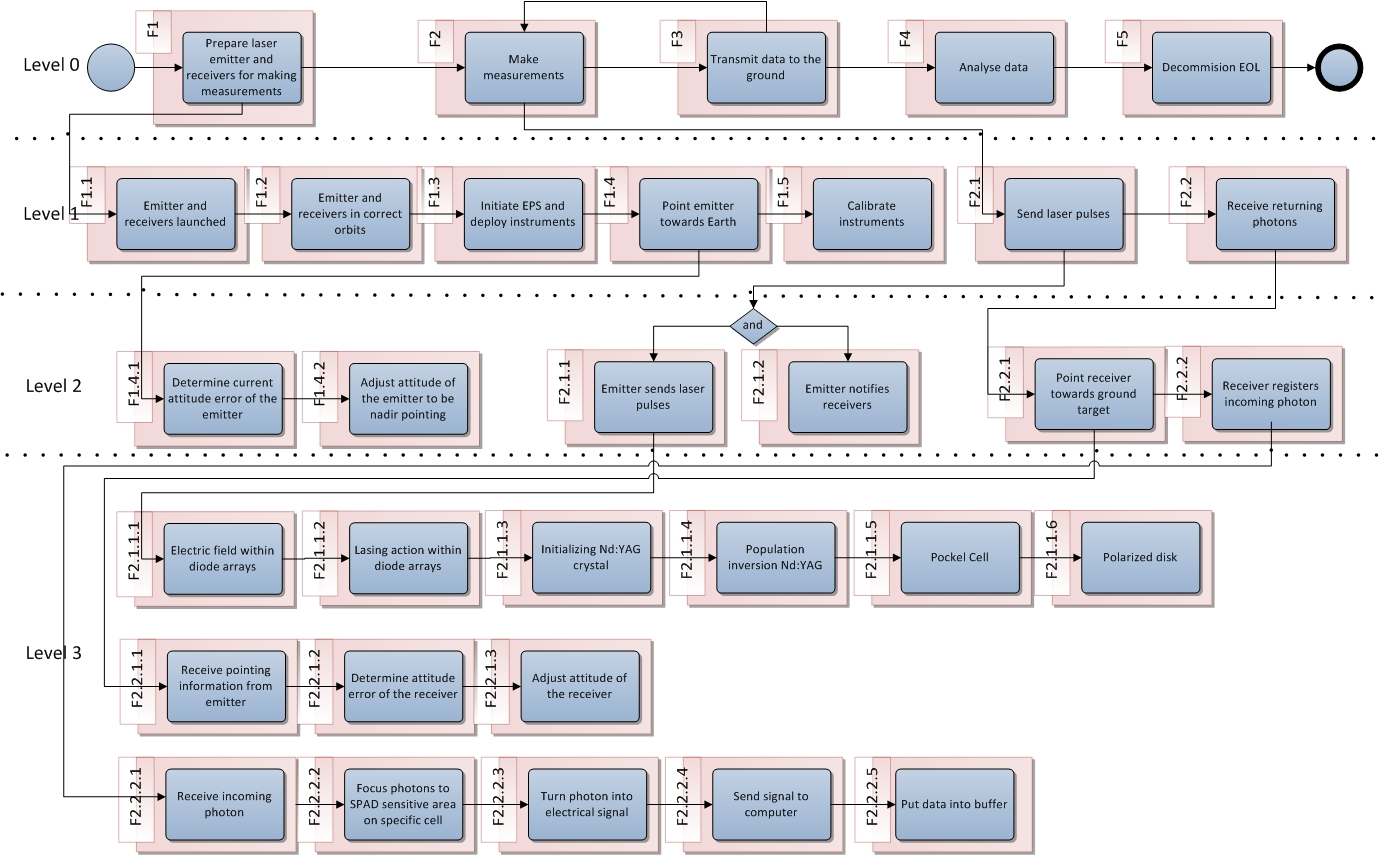
\includegraphics[width=1.3\textheight]{chapters/img/FFD1.jpg}
\caption{Functional Flow Diagram part 1(F1 and F2 detail) of the Laser Swarm mission}
\label{FFD1}
\end{figure}
\end{landscape}

\begin{landscape}
\begin{figure}[ht!]
\centering
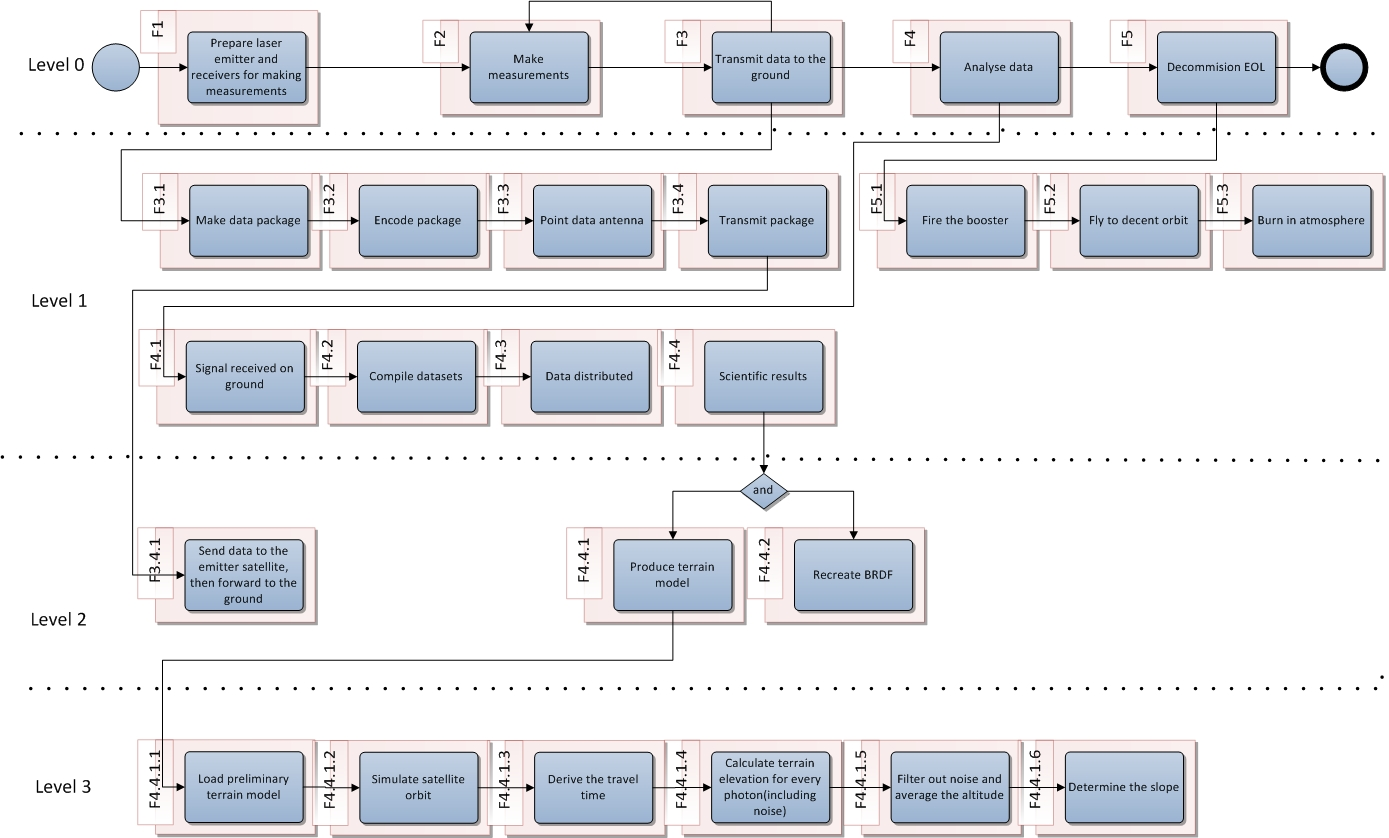
\includegraphics[width=1.3\textheight]{chapters/img/FFD2.jpg}
\caption{Functional Flow Diagram part 2(F3, F4 and F5 detail) of the Laser Swarm mission}
\label{FFD2}
\end{figure}
\end{landscape}

\section{Functional Breakdown Structure}
\label{section_FBS}
The \ac{FBS} shows the functions the system needs to perform, broken up in subtasks from other functions. The schematic representation can be found in figure \ref{FBS} on page \pageref{FBS}.

The main function for the system is to be able to get scientific results for producing the terrain model and recreating the \acs{BRDF}, which is the reason for making the measurements. To be able to produce the terrain model measurements need to be made, the data needs to be transmitted to the ground and needs to be analyzed. Because the mission has to be sustainable, the satellites are decommissioned at the end of their life, so they will not pose a threat to other satellites.


The measurements depend on laser pulses to be transmitted, reflected photons to be detected and the emitter and receivers to be in the correct orbit with the instruments calibrated. For the data to be transmitted to Earth, the antenna needs to be pointed to the ground station and the data package has to be transmitted. Data analysis depends on the data to be received on the ground and the distribution between the research institutes.

Before the emitter satellite can send down laser pulses to Earth, the laser emitter on board needs to be pointed at nadir. To receive the reflected photons the receiver satellite has to point its receiver payload at the ground target and has to register the incoming photons. For the data package to be transmitted, data is put into a buffer, a data package is made, the package is coded and the receiver satellite sends the data to the emitter satellite, which in turn forwards it to Earth. It is important to have the \ac{EPS} properly functioning and instruments deployed before they can be calibrated.

Determining the attitude error of the emitter satellite and adjusting  it accordingly is required to point the emitter payload towards Earth. When an incoming photon is received, it is transformed into a digital signal and the signal is sent to the on-board computer so the photon is registered. For the receiver payload to be pointed at the ground target, the emitter satellite needs to notify the receiver satellites it has sent pulses. The receiver satellite needs to receive the message, interpret it, determine attitude error and adapt accordingly to make sure that data gathering will be carried out properly. 

\begin{landscape}
\begin{figure}[ht!]
\centering
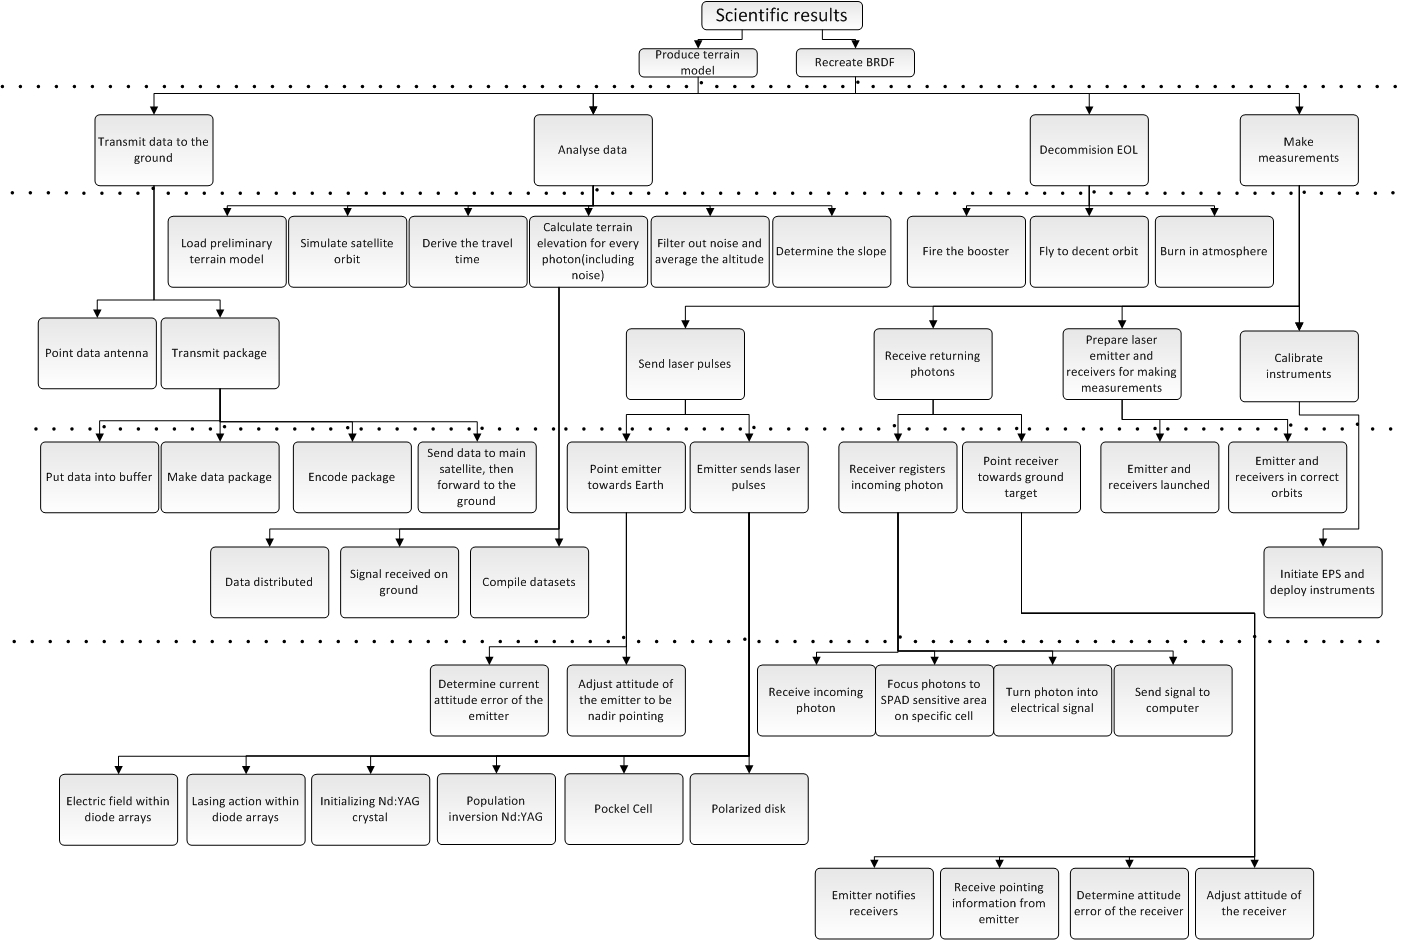
\includegraphics[width=1.3\textheight]{chapters/img/FBD.jpg}
\caption{Functional breakdown structure of the Laser Swarm mission}
\label{FBS}
\end{figure}
\end{landscape}


